\documentclass[english,master,buw]{webisthesis} % Weimar
% \documentclass[german,bachelor,fsu]{webisthesis} % Jena
% \documentclass[german,bachelor,ul]{webisthesis} % Leipzig
% \documentclass[german,master,buw,web]{webisthesis} % Weimar, for web page
% \documentclass[german,bachelor,fsu,web]{webisthesis} % Jena, for web page
% \documentclass[german,bachelor,ul,web]{webisthesis} % Leipzig, for web page
%
% Non-default programme
% ---------------------
% \documentclass[english,master,buw]{webisthesis}\global\thesisprogramme{Human-Computer Interaction}
% \documentclass[english,master,buw]{webisthesis}\global\thesisfrontpagefaculty{Faculty of Civil Engineering/Faculty of Media}\global\thesisprogramme{Digital Engineering}
% \documentclass[german,bachelor,buw]{webisthesis}\global\thesisprogramme{Informatik\\Schwerpunkt Medieninformatik}
% \documentclass[german,bachelor,buw]{webisthesis}\global\thesisprogramme{Informatik\\Schwerpunkt Security and Data Science}
%
% When you change the language, pdflatex may halt on recompilation.
% Just hit enter to continue and recompile again. This should fix it.


%
% Values
% ------
\ThesisSetTitle{
    Generative Agents School:\\
    The Impact of Thuringian Government Programs on Generative Students
}
\ThesisSetKeywords{These, are, my, Keywords} % only for PDF meta attributes

\ThesisSetAuthor{Julian Klüber}
\ThesisSetAuthorSecond{Varuna Sethuraman}
\ThesisSetStudentNumber{129164}
\ThesisSetStudentNumberSecond{000000}

\ThesisSetSubmissionDate{18}{8}{2026}

\usepackage{graphicx}
\usepackage{pdfpages}

%
% Suggested Packages
% ------------------
\usepackage[style=alphabetic,natbib=true,backend=biber]{biblatex}
\addbibresource{literature.bib}

\usepackage{booktabs}
%    For tables ``looking the right way''.
%
\usepackage{tabularx}
\usepackage{multirow}
\usepackage{longtable}
\usepackage{enumitem}  % For bullet point formatting
\usepackage{needspace} % Prevents isolated category titles at page bottoms
\usepackage{pdflscape} % Optional: if you decide to view it horizontally
%    Enables tables with columns that automatically fill the page width.
%
% \usepackage[ruled,algochapter]{algorithm2e}
%    A package for pseudo code algorithms.
%
\usepackage{amsmath}
%    For tabular-style formatting of mathematical environments.
%

\usepackage{fontawesome}
%    For lots of awesome glyphs: https://mirror.physik.tu-berlin.de/pub/CTAN/fonts/fontawesome/doc/fontawesome.pdf

%
% Commenting (by your supervisor)
% -------------------------------
\usepackage{xcolor}
\usepackage{soul}
\newcommand{\bscom}[2]{%
  % #1 Original text.
  % #2 Replacement text.
    \st{\scriptsize\,#1}{\color{blue}\scriptsize\,#2}%
  }

\usepackage{titlesec}

\titleformat{\chapter}[hang]
  {\normalfont\huge\bfseries} % Formatting of the heading
  {\thechapter}               % Chapter number (prints "1" instead of "Chapter 1")
  {1em}                       % Space between number and title
  {}                          % Code before the title text

% Create links in the pdf document
% Hyperref has some incompatibilities with other packages
% Some other packages must be loaded before, some after hyperref
% Additional options to the hyperref package can be provided in the braces [], like in
% \usehyperref[backref] % This will add back references in the bibliography that some people like ... some don't ... so better ask your supervisor ;-)
\usehyperref

\begin{document}
\begin{frontmatter}
\begin{abstract}
This is the \LaTeX{} template for Bachelor and Master theses at Webis. This template contains several hints and conventions on how to structure a thesis, how to cite the work of others, and how to display your results besides plain text. 
\end{abstract}

\tableofcontents

% \chapter*{Acknowledgements} % optional
% I thank the authors of the webisthesis template for their excellent work!

% \listoffigures % optional, usually not needed

% \listoftables % optional, usually not needed

% \listofalgorithms % optional, usually not needed
%    requires package algorithm2e

% optional: list of symbols/notation (e.g., using the nomencl package) but usually not needed
\end{frontmatter}

\chapter{Introduction}
\label{introduction}

Society relies on education to transmit culture, maintain social framework, and cultivate engaged citizens~\cite{dewey:1916, bourdieu:1970}. Modern states formalise this process through public schooling, establishing standardised environments wherein children acquire the necessary competencies to participate in democratic life~\cite{dewey:1916}. 

However, formal education is inherently value-laden; decisions regarding what knowledge is essential and how classrooms should be governed are fundamental political questions~\cite{apple:2004}. 
In democratic systems such as Germany, state governments determine educational policies, curriculum frameworks, and school structures. 
Political parties hold sharply contrasting visions of educational priorities.
In practice, democratic coalition building forces political parties to compromise, meaning that pure ideological platforms are rarely observed in isolation within real-world classrooms. 
Evaluating how these uncompromised party programmes independently affect student well-being, social dynamics, and personality development presents a methodological challenge.

To overcome real-world policy blurring and isolate party-specific educational visions, the \textit{Generative Agents School}\footnote{\faGithub\ Code base: \href{https://github.com/JKlueber/generative_agents_school}{github.com/JKlueber/generative\_agents\_school}} constructs a simulated educational environment using the generative agents architecture introduced by~\citeauthor{park:2023} \cite{park:2023}. 
By instantiating autonomous LLM-driven agents within a controlled sandbox environment, we translate the distinct educational programmes of \textit{Die Linke}, \textit{SPD}, \textit{B\"undnis 90/Die Gr\"unen}, \textit{CDU}, and \textit{AfD} into explicit school rules and classroom curricula. 
Holding the baseline environment constant, we fork a single initial state into five parallel timelines, simulating a school day under each party's distinct regime. 
To evaluate the impact of each party framework, we administer the Big Five Inventory-2 (BFI-2) to student agents before the simulation fork and after the completion of the simulated school day to assess shifts in their personality traits.
\chapter{Related Work} \label{relatedWork}
\chapter{Setting the Environment} \label{settingTheEnvironment}
\chapter{Analysis}

\subsection{Direction and consistency across environments}

Two patterns stand out. First, Open-Mindedness rises significantly in every single party environment ($\Delta$ between 0.65 and 0.83, all $p_t<0.05$), making it the only domain with a uniformly significant effect across the full political spectrum represented in the simulation. Second, every environment moves every domain in the same direction: all five parties increase Extraversion, Agreeableness, Conscientiousness, and Open-Mindedness relative to base, and all five decrease Neg.\ Emotionality. No party reverses the sign of any domain. This uniformity suggests that part of the measured effect may be attributable to a general simulation exposure effect, meaning agents becoming more socially confident and less anxious simply from having lived through a structured school day and interacted with peers, independent of which party's policies governed that day rather than a purely party-specific ideological effect. We return to this as a limitation in Chapter~\ref{limitations}.

Where the parties differ is in magnitude and in which domains cross the significance threshold (Appendix~\ref{appendix:paired_stats}):

\begin{itemize}
\item \textbf{Linke} produces the largest Agreeableness increase of any party ($\Delta=0.56$, $d=3.56$) and the largest decrease in Neg.\ Emotionality ($\Delta=-0.31$, $d=-2.98$), both significant. This is consistent with Die Linke's programme of non-selective schooling, individualised feedback instead of grades, and reduced homework (Section~1), which removes several common sources of peer competition and performance pressure.
\item \textbf{Gr\"une} is the only other party with a significant Neg.\ Emotionality decrease ($\Delta=-0.25$, $d=-3.66$) alongside a significant Agreeableness gain, matching its stated emphasis on inclusion and modern, participatory pedagogy.
\item \textbf{SPD} shows the strongest Open-Mindedness effect of all five parties ($\Delta=0.83$) and is one of only two environments with a significant Extraversion increase ($\Delta=0.21$, $p_t=0.030$), broadly consistent with its focus on educational mobility and opportunity.
\item \textbf{AfD} produces significant increases in Extraversion ($\Delta=0.44$, the largest of any party), Agreeableness, and Open-Mindedness. This is a counter-intuitive result given the party's traditional, discipline-oriented programme, and is discussed further in Chapter~\ref{limitations}.
\item \textbf{CDU} is the environment with the fewest significant shifts, only Open-Mindedness reaches significance. Point estimates for Conscientiousness (0.35) and Extraversion (0.38) are comparable in size to the other parties, but higher within-agent variance (larger $sd_{\Delta}$) keeps them below the significance threshold. This relative "flatness" is at least directionally consistent with a programme built around stability, performance standards, and the traditional multi-track structure.
\end{itemize}

Conscientiousness is the one domain that never reaches significance in any environment, despite positive point estimates throughout (0.31--0.40). Given paired Cohen's $d$ values in the 0.6--1.0 range, this looks like a power problem rather than a null effect: the true shift is plausibly non-zero, but $n=4$ students is not enough to detect a medium effect size reliably.

\section{Individual-Level Variation}
\label{sec:individual-level}

Group means can mask substantial disagreement between agents. Figure~\ref{fig:individual-heatmap} breaks the domain shifts down by agent (including the teacher, Katharina Weber) and environment.

\begin{figure}[htbp]
\centering
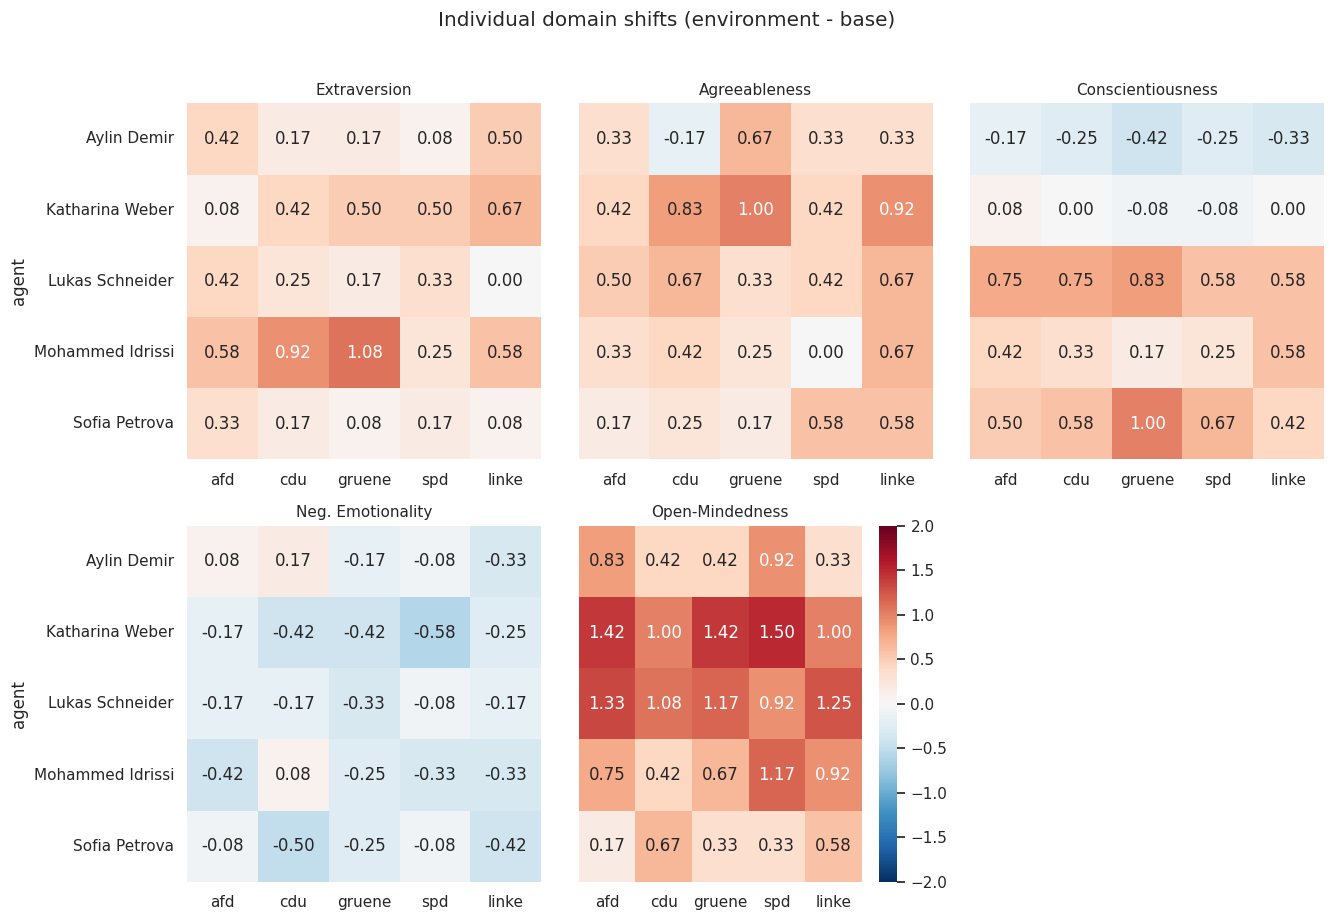
\includegraphics[width=\textwidth]{figures/individual_shift_heatmap.png}
\caption{Individual domain shifts (environment $-$ base) by agent. Katharina Weber is the teacher agent; the remaining four rows are the students used in Table~\ref{tab:paired-stats}.}
\label{fig:individual-heatmap}
\end{figure}

\begin{figure}[htbp]
\centering
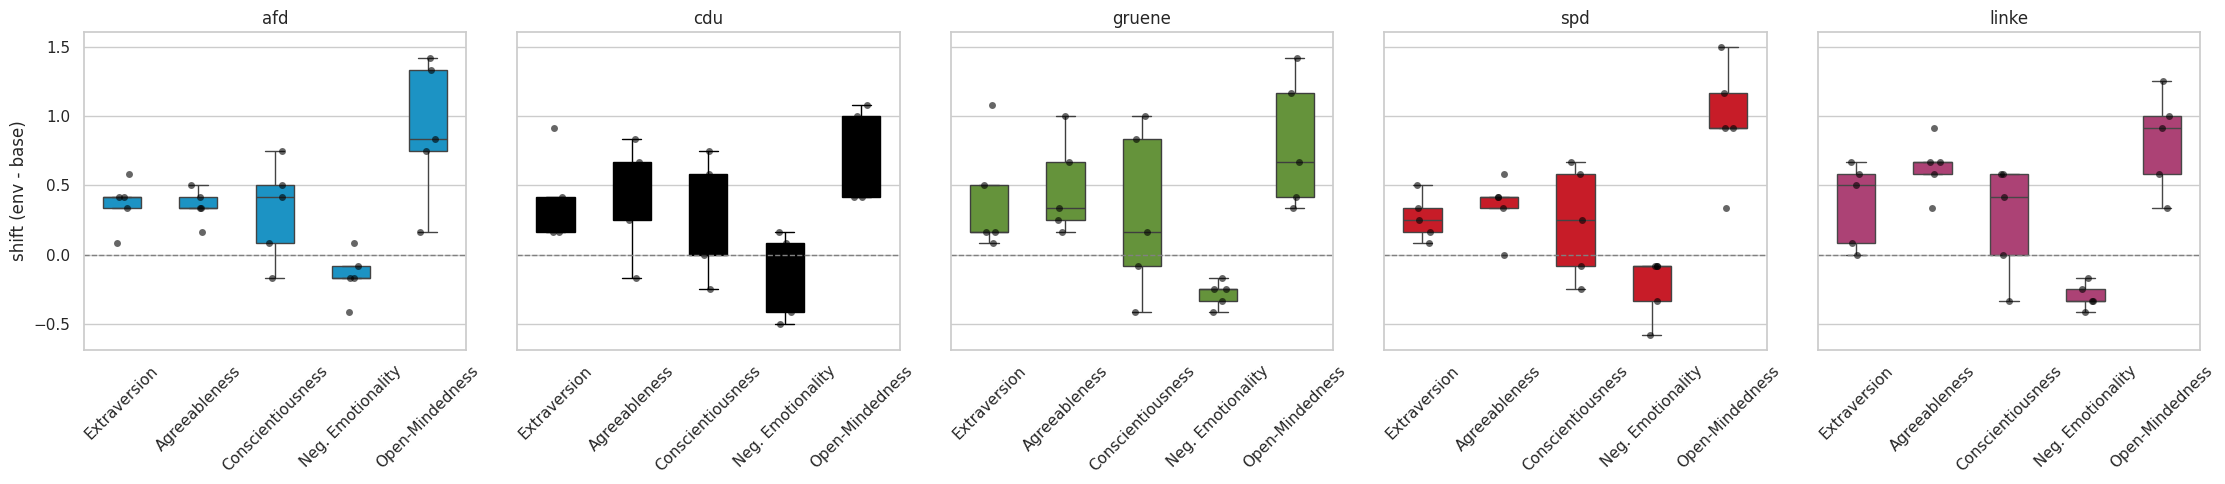
\includegraphics[width=\textwidth]{figures/spread_boxplot.png}
\caption{Spread of individual student shifts per domain, one panel per environment.}
\label{fig:spread}
\end{figure}

Three observations follow from the individual-level view. First, the teacher
agent, Katharina Weber, consistently shows the \emph{largest} Open-Mindedness
shift of any agent in every environment (1.00--1.50), well above the student
range (0.33--1.33). Since her role and daily schedule were rewritten for
each party to reflect that party's pedagogical philosophy, this is expected:
she is the agent most directly exposed to the ideological content of each
environment, and it registers most strongly on her open-mindedness score.

Second, the boxplots in Figure~\ref{fig:spread} show that
\textbf{Conscientiousness has the widest interquartile spread of any domain
in most environments} (e.g.\ CDU ranges from about $-0.5$ to $+0.75$), which
explains why it never reaches significance in Table~\ref{tab:paired-stats}
despite consistently positive medians: individual agents respond quite
differently to the same environment. Neg.\ Emotionality and Open-Mindedness,
by contrast, show comparatively tight, one-sided distributions (nearly all
individual shifts negative for Neg.\ Emotionality and positive for
Open-Mindedness), which is why those two domains yield the clearest
significant effects.

Third, no single student is a uniform outlier: each of the four students
(Sofia Petrova, Mohammed Idrissi, Lukas Schneider, Aylin Demir) shows at
least one domain/environment combination with a shift near zero or slightly
negative, even in domains where the group mean is strongly positive, e.g.\
Aylin Demir's Conscientiousness shift is negative in four of the five
environments while the group mean is positive throughout. This indicates
that the group-level effects in Section~4.1 are driven by a majority
tendency rather than by unanimous agreement among agents.

\section{Facet-Level Detail}

Figure~\ref{fig:facet-radar} disaggregates the five domains into their 15
constituent BFI-2 facets, plotting the group-mean facet profile for each
environment against the base measurement.

\begin{figure}[htbp]
\centering
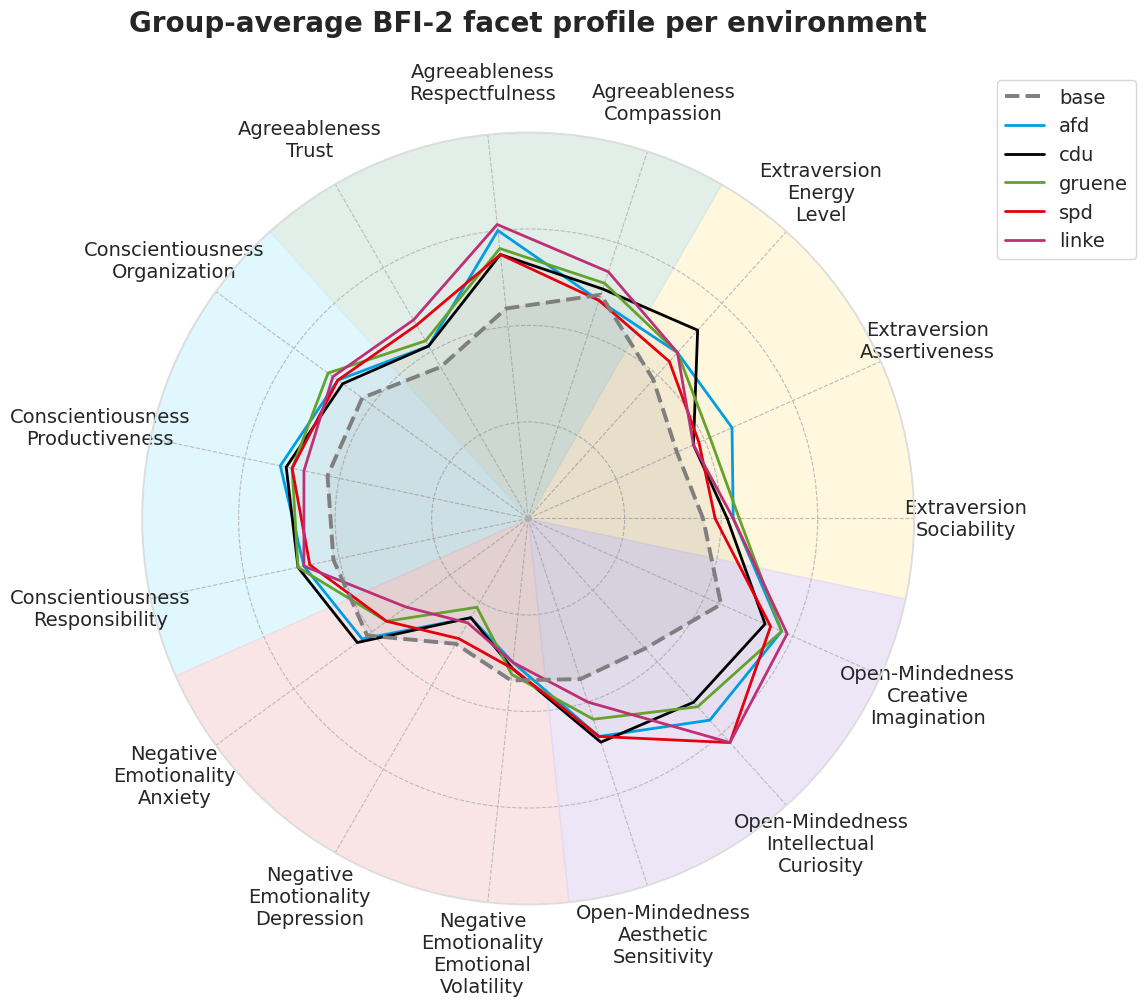
\includegraphics[width=0.75\textwidth]{figures/facet_radar.png}
\caption{Group-average BFI-2 facet profile per environment (15 facets, base vs.\ five party environments).}
\label{fig:facet-radar}
\end{figure}

The facet view shows that the domain-level Open-Mindedness effect is carried
primarily by \emph{Intellectual Curiosity} and \emph{Aesthetic Sensitivity},
which separate most clearly from the base profile across all five
environments, while \emph{Creative Imagination} shows a smaller gap. Within
Agreeableness, \emph{Respectfulness} shows the largest and most consistent
separation from base of the three facets — plausibly reflecting that a full
day inside any of the five structured party environments, each with its own
explicit classroom rules, increases agents' expressed respect for
those rules and for the teacher — while \emph{Trust} moves by comparatively
less. Within Conscientiousness, \emph{Organization} separates from base more
than \emph{Productiveness} or \emph{Responsibility}, consistent with the
domain-level result being real but individually noisy (Section~4.2). The
Negative Emotionality facets move together as a block, with \emph{Depression}
showing the clearest environment-vs-base gap and \emph{Anxiety} the
smallest, matching the domain-level finding that the overall Neg.\
Emotionality decrease is modest but directionally consistent.
\chapter{Discussion}
\label{discussion}

Across all five simulated party environments, student agents' expressed Big Five profiles shifted in the same direction with higher Extraversion, higher Agreeableness, higher Conscientiousness, higher Open-Mindedness and lower Negative Emotionality relative to the pre-simulation baseline. Reliable statistical significance is concentrated in Open-Mindedness (all five parties), Agreeableness (AfD, Gr\"une, Linke), Extraversion (AfD, SPD), and Neg.\ Emotionality (Gr\"une, Linke). 

Linke produced the strongest pro-social effect (largest Agreeableness gain, largest Neg.\ Emotionality drop), consistent with its low-pressure, non-selective programme, while CDU produced the fewest significant shifts overall, consistent with its stability- and discipline-oriented programme. SPD's environment stood out for the largest Open-Mindedness gain, and AfD unexpectedly combined the largest Extraversion gain with significant Agreeableness and Open-Mindedness gains despite its traditional, discipline-focused platform.

This last result, together with the fact that no domain reverses sign in any environment, is a reason for caution rather than a straightforward finding about AfD's programme specifically. 

Three limitations must be considered when interpreting these results:

\begin{enumerate}
\item \textbf{Sample size.} The paired analysis rests on $n=4$ students per environment. This may be enough to detect very large effects (Open-Mindedness, $d>1.6$ throughout) but it is underpowered for the medium effects seen in Conscientiousness, and it limits the Wilcoxon test to a small set of possible $p$-values, several of which never reach $p<0.05$ regardless of effect size.
\item \textbf{Uniform direction across parties.} Every environment shifted every domain the same way, which is consistent with a general "day in a structured simulated school with peers" effect that is at least partly independent of the specific party programme. The between-party differences we report are therefore best read as differences in magnitude on top of a shared baseline exposure effect, not as fully independent, party-caused effects.
\item \textbf{Time and cost limits.} To run the simulation for a school day until 12:00 PM, each environment took approximately 4 hours, because every time the agents reflect or converse, they must generate multiple LLM responses. Those LLM calls are expensive, and the simulation is time-consuming. This limits the number of agents and the number of days we can simulate, which in turn limits statistical power and the ability to observe longer-term effects.
\end{enumerate}

Future work could extend the simulation to multiple school days per environment to test if party-specific differences grow relative to the shared baseline effect, and increase the number of student agents per timeline to improve statistical power. However, this depends on whether the simulation time and cost can be reduced.

\printbibliography

\appendix
% Suppresses all subsequent chapters and sections from the Table of Contents
\addtocontents{toc}{\protect\setcounter{tocdepth}{-1}}

\chapter{Appendix}\label{appendix}

\section{Party Policy Comparison}\label{appendix:party_policies}
\begingroup
\scriptsize % Keeps text clean and easily scannable

\begin{longtable}{>{\bfseries\raggedright\arraybackslash}p{0.22\textwidth} 
                  >{\raggedright\arraybackslash}p{0.73\textwidth}}

% Caption for the FIRST page
\caption{Comparison of Thuringian Party Positions on Educational Policy} \label{tab:party_comparison} \\
\toprule
{\normalsize\bfseries Party} & {\normalsize\bfseries Key Program Points} \\
\midrule
\endfirsthead

% Header for SUBSEQUENT pages
\multicolumn{2}{c}{\tablename\ \thetable\ -- \textit{Continued from previous page}} \\ [0.5ex]
\toprule
{\normalsize\bfseries Party} & {\normalsize\bfseries Key Program Points} \\
\midrule
\endhead

% Footer on intermediate pages
\bottomrule
\multicolumn{2}{r}{\textit{Continued on next page}} \\
\endfoot

% Final footer on last page
\bottomrule
\endlastfoot

% ==================== CATEGORY 1 ====================
\multicolumn{2}{c}{\normalsize\bfseries 1. School System \& Structure} \\* [0.5ex] 
\hline \noalign{\vskip 0.8ex}

Die Linke & 
\begin{itemize}[leftmargin=*, nosep]
  \item \textbf{School Type:} Expansion of the \emph{Gemeinschaftsschule}\footnote{\textbf{Gemeinschaftsschule:} Comprehensive school model in Germany where children of all ability levels learn together (grades 1--10/13).}.
  \item \textbf{All-day \& After-school:} Expansion of all-day offers; abolition of after-school care (\emph{Hort}\footnote{\textbf{Hort:} After-school care program located at primary schools.}) fees (gradual expansion to grades 5--6); full-time contracts for educators.
  \item \textbf{Administration \& Participation:} State-wide hiring of school administration assistants; expansion of democratic student representation.
\end{itemize} \\ \hline \noalign{\vskip 0.5ex}

SPD & 
\begin{itemize}[leftmargin=*, nosep]
  \item \textbf{School Type:} Priority on \emph{Gemeinschaftsschule}.
  \item \textbf{All-day:} Genuine all-day concept (alternating instruction, leisure, and recovery throughout the day).
  \item \textbf{Administration \& Participation:} Hiring of administration assistants; student participation (50\% of school conference based on Berlin model).
\end{itemize} \\ \hline \noalign{\vskip 0.5ex}

Bündnis 90/Die Grünen & 
\begin{itemize}[leftmargin=*, nosep]
  \item \textbf{School Type:} \emph{Gemeinschaftsschule}.
  \item \textbf{All-day \& Relief:} Expansion of all-day schools; fee-free school transport and free learning materials.
  \item \textbf{Support:} Guaranteed school social work at every school and strengthening school psychology.
\end{itemize} \\ \hline \noalign{\vskip 0.5ex}

CDU & 
\begin{itemize}[leftmargin=*, nosep]
  \item \textbf{School Type:} Retention of tracked school system; state-wide retention of special schools (\emph{Förderschulen}\footnote{\textbf{Förderschule:} Specialized school for children with physical, mental, or learning disabilities.}).
  \item \textbf{All-day:} Retention of all-day offers alongside complete abolition of after-school care (\emph{Hort}) fees.
\end{itemize} \\ \hline \noalign{\vskip 0.5ex}

AfD & 
\begin{itemize}[leftmargin=*, nosep]
  \item \textbf{School Type:} Commitment to tracked system; upgrading \emph{Regelschule}\footnote{\textbf{Regelschule:} Secondary track in Thuringia combining vocational/general education.} and aligning \emph{Gymnasium}\footnote{\textbf{Gymnasium:} Highest academic secondary track leading to university qualification.} to university entry.
  \item \textbf{All-day:} Rejection of mandatory all-day schools; voluntary afternoon care.
  \item \textbf{Administration:} State-wide administrative assistants to relieve teachers.
\end{itemize} \\ \tabularnewline [2ex]

% ==================== CATEGORY 2 ====================
\multicolumn{2}{c}{\normalsize\bfseries 2. Grading \& Assessment} \\* [0.5ex] 
\hline \noalign{\vskip 0.8ex}

Die Linke & 
\begin{itemize}[leftmargin=*, nosep]
  \item \textbf{Grading:} Advance assessment without numerical grades; abolition of grades in PE, music, and art.
  \item \textbf{Graduation \& Qualifications:} Abolition of Special Performance Assessment (\emph{BLF}\footnote{\textbf{BLF:} Besondere Leistungsfeststellung exam at end of 10th grade in Gymnasium.}) at \emph{Gymnasien}; automatic acquisition of intermediate certificate (\emph{Realschulabschluss}\footnote{\textbf{Realschulabschluss:} Intermediate school leaving certificate after 10th grade.}) upon promotion to grade 11.
\end{itemize} \\ \hline \noalign{\vskip 0.5ex}

SPD & 
\emph{(No specific details provided in the text)} \\ \hline \noalign{\vskip 0.5ex}

Bündnis 90/Die Grünen & 
\begin{itemize}[leftmargin=*, nosep]
  \item \textbf{Grading \& Pressure:} Individual support over performance pressure; written evaluations instead of numerical grades in PE, art, and music.
  \item \textbf{Graduation \& Retention:} Abolishing \emph{BLF} (automatic certificate on grade 11 promotion); abolishing grade retention in favor of targeted support.
\end{itemize} \\ \hline \noalign{\vskip 0.5ex}

CDU & 
\begin{itemize}[leftmargin=*, nosep]
  \item \textbf{Grading \& Retention:} Reintroduction of conduct grades (\emph{Kopfnoten}\footnote{\textbf{Kopfnoten:} Conduct grades assessing behavior, effort, participation, orderliness.}: behavior, effort, participation, orderliness); binding promotion decisions starting grade 2.
  \item \textbf{Graduation \& Qualifications:} Retaining \emph{BLF} in grade 10 as preparation for \emph{Abitur}\footnote{\textbf{Abitur:} Final qualification exam granting university entry.}.
\end{itemize} \\ \hline \noalign{\vskip 0.5ex}

AfD & 
\begin{itemize}[leftmargin=*, nosep]
  \item \textbf{Grading \& Retention:} Retaining/reintroducing classic grades starting grade 2 and conduct grades (\emph{Kopfnoten}); enabling grade repetition in every grade level.
  \item \textbf{Graduation \& Qualifications:} Retaining \emph{BLF} in grade 10, qualifying it as full intermediate certificate (\emph{Realschulabschluss}).
\end{itemize} \\ \tabularnewline [2ex]

% ==================== CATEGORY 3 ====================
\multicolumn{2}{c}{\normalsize\bfseries 3. Instruction \& Pedagogical Concepts} \\* [0.5ex] 
\hline \noalign{\vskip 0.8ex}

Die Linke & 
\begin{itemize}[leftmargin=*, nosep]
  \item \textbf{Pedagogical Assistance:} Permanent hiring and staff expansion of pedagogical assistants.
  \item \textbf{School Life \& Practice:} Developing individual school concepts involving parents/students; expanding polytechnic/practical learning.
\end{itemize} \\ \hline \noalign{\vskip 0.5ex}

SPD & 
\begin{itemize}[leftmargin=*, nosep]
  \item \textbf{Daily Schedule:} School start no earlier than 09:00 AM; shortening instructional units to 45--60 mins.
  \item \textbf{Civic Education:} Expansion of social studies instruction; cross-curricular democratic orientation.
\end{itemize} \\ \hline \noalign{\vskip 0.5ex}

Bündnis 90/Die Grünen & 
\begin{itemize}[leftmargin=*, nosep]
  \item \textbf{Content \& Curricula:} Cross-curricular teaching and modern curricula (mental health, nutrition); reviewing materials for discrimination.
  \item \textbf{Learning Forms:} Reducing homework; strengthening learning outside school; joint dialogue module for ethics/religion.
\end{itemize} \\ \hline \noalign{\vskip 0.5ex}

CDU & 
\begin{itemize}[leftmargin=*, nosep]
  \item \textbf{Language \& Values:} Standard spelling rules (ban on gender-neutral special characters); strengthening democracy/values education and culture of remembrance.
  \item \textbf{Practice \& STEM:} Strengthening STEM (\emph{MINT}\footnote{\textbf{MINT:} German equivalent of STEM (Math, CS, Sciences, Tech).}) subjects; introducing state-wide ``Day in Practice''.
\end{itemize} \\ \hline \noalign{\vskip 0.5ex}

AfD & 
\begin{itemize}[leftmargin=*, nosep]
  \item \textbf{Orientation \& Values:} Knowledge-based uniform curricula; teaching secondary virtues (punctuality, orderliness).
  \item \textbf{Instructional Rules:} Strict ban on gender-neutral language; enforcement of neutrality mandate (\emph{Beutelsbacher Konsens}\footnote{\textbf{Beutelsbacher Konsens:} Guidelines mandating political neutrality in education.}); rejection of Islamic religious education.
\end{itemize} \\ \tabularnewline [2ex]

% ==================== CATEGORY 4 ====================
\multicolumn{2}{c}{\normalsize\bfseries 4. Digitalization \& Media} \\* [0.5ex] 
\hline \noalign{\vskip 0.8ex}

Die Linke & 
\begin{itemize}[leftmargin=*, nosep]
  \item \textbf{Access \& Support:} Genuine free access to learning materials (analog \& digital).
  \item \textbf{Media Literacy:} Media concepts at every school; critical social media instruction from entry level; expanding technical support.
\end{itemize} \\ \hline \noalign{\vskip 0.5ex}

SPD & 
\begin{itemize}[leftmargin=*, nosep]
  \item \textbf{Access \& Competence:} Free learning materials including digital end-user devices.
  \item \textbf{Educational Goal:} Fostering ``digital resilience'' and critical media use.
\end{itemize} \\ \hline \noalign{\vskip 0.5ex}

Bündnis 90/Die Grünen & 
\begin{itemize}[leftmargin=*, nosep]
  \item \textbf{Infrastructure:} Guaranteeing digital device for every child; increasing infrastructure investments.
  \item \textbf{Usage:} Expanding CS and media education; no blanket smartphone ban (determined with students).
\end{itemize} \\ \hline \noalign{\vskip 0.5ex}

CDU & 
\begin{itemize}[leftmargin=*, nosep]
  \item \textbf{Equipment:} Equipping students from grade 5 with loan devices via special funding.
  \item \textbf{Support \& Teaching:} Deploying ``digital caretakers'' for IT; mandatory AI/digital training in teacher education.
\end{itemize} \\ \hline \noalign{\vskip 0.5ex}

AfD & 
\begin{itemize}[leftmargin=*, nosep]
  \item \textbf{Stance:} ``Digitalization with a sense of proportion''; rejecting replacement of teachers by digital media.
  \item \textbf{AI \& Media:} Pragmatic approach to AI (ChatGPT) in teaching instead of bans; educating about risks.
\end{itemize} \\ \tabularnewline [2ex]

% ==================== CATEGORY 5 ====================
\multicolumn{2}{c}{\normalsize\bfseries 5. Inclusion \& Language Support} \\* [0.5ex] 
\hline \noalign{\vskip 0.8ex}

Die Linke & 
\begin{itemize}[leftmargin=*, nosep]
  \item \textbf{Inclusion:} Expanding right to inclusive education via modern settings and professional development.
  \item \textbf{Language Support:} Overall concept for non-native German speakers focusing on German as Second Language (\emph{DaZ}\footnote{\textbf{DaZ:} German as a Second Language instruction programs.}) teachers.
\end{itemize} \\ \hline \noalign{\vskip 0.5ex}

SPD & 
\begin{itemize}[leftmargin=*, nosep]
  \item \textbf{Support:} Multi-professional teams on-site (special education teachers, \emph{DaZ} teachers, social workers).
\end{itemize} \\ \hline \noalign{\vskip 0.5ex}

Bündnis 90/Die Grünen & 
\begin{itemize}[leftmargin=*, nosep]
  \item \textbf{Inclusion:} Improving joint learning of children with and without disabilities; trust teachers as anti-discrimination officers (\emph{SAVE}\footnote{\textbf{SAVE-Beauftragte:} School officers designated for Anti-discrimination, Diversity, and Empowerment.}).
  \item \textbf{Language Support:} Expanding capacities for \emph{DaZ}.
\end{itemize} \\ \hline \noalign{\vskip 0.5ex}

CDU & 
\begin{itemize}[leftmargin=*, nosep]
  \item \textbf{Inclusion \& Special Schools:} Parental school choice rights remain; state-wide retention of special schools (\emph{Förderschulen}).
  \item \textbf{Language Support:} Mandatory language tests prior to enrollment; creation of support classes.
\end{itemize} \\ \hline \noalign{\vskip 0.5ex}

AfD & 
\begin{itemize}[leftmargin=*, nosep]
  \item \textbf{Inclusion \& Special Schools:} Priority on retaining and expanding special schools (\emph{Förderschulen}).
  \item \textbf{Language Support:} Mandatory preparatory classes with testing for foreign children lacking German skills.
\end{itemize} \\ 
\bottomrule
\end{longtable}

\endgroup

\newpage
\section{Big Five Personality Shift Analysis}\label{appendix:paired_stats}
\begin{table}[htbp]
\centering
\small
\caption{Paired shift statistics per environment $\times$ domain ($n=4$ students). $\Delta$ = mean shift (environment $-$ base), $d$ = paired Cohen's $d$, $p_t$ = paired $t$-test $p$-value, $p_W$ = Wilcoxon $p$-value. Bold rows are significant at $p_t<0.05$.}
\label{tab:paired-stats}
\begin{tabular}{llrrrrr}
\toprule
Domain & Party & $\Delta$ & $d$ & $t$ & $p_t$ & $p_W$ \\
\midrule
\multirow{5}{*}{Extraversion}
 & \textbf{AfD}   & \textbf{0.438} & \textbf{4.18} & \textbf{8.35} & \textbf{0.004} & 0.125 \\
 & CDU            & 0.375 & 1.03 & 2.07 & 0.131 & 0.125 \\
 & Gr\"une        & 0.375 & 0.79 & 1.58 & 0.212 & 0.125 \\
 & \textbf{SPD}   & \textbf{0.209} & \textbf{1.95} & \textbf{3.89} & \textbf{0.030} & 0.125 \\
 & Linke          & 0.292 & 1.00 & 1.99 & 0.140 & 0.250 \\
\midrule
\multirow{5}{*}{Agreeableness}
 & \textbf{AfD}   & \textbf{0.333} & \textbf{2.45} & \textbf{4.90} & \textbf{0.016} & 0.125 \\
 & CDU            & 0.292 & 0.83 & 1.66 & 0.195 & 0.250 \\
 & \textbf{Gr\"une} & \textbf{0.354} & \textbf{1.62} & \textbf{3.24} & \textbf{0.048} & 0.125 \\
 & SPD            & 0.333 & 1.36 & 2.72 & 0.073 & 0.250 \\
 & \textbf{Linke} & \textbf{0.562} & \textbf{3.56} & \textbf{7.13} & \textbf{0.006} & 0.125 \\
\midrule
\multirow{5}{*}{Conscientiousness}
 & AfD            & 0.375 & 0.97 & 1.93 & 0.149 & 0.250 \\
 & CDU            & 0.354 & 0.81 & 1.62 & 0.204 & 0.250 \\
 & Gr\"une        & 0.396 & 0.61 & 1.22 & 0.311 & 0.375 \\
 & SPD            & 0.312 & 0.75 & 1.50 & 0.230 & 0.375 \\
 & Linke          & 0.312 & 0.71 & 1.43 & 0.249 & 0.250 \\
\midrule
\multirow{5}{*}{Neg.\ Emotionality}
 & AfD            & $-$0.146 & $-$0.70 & $-$1.40 & 0.257 & 0.375 \\
 & CDU            & $-$0.104 & $-$0.35 & $-$0.70 & 0.537 & 0.750 \\
 & \textbf{Gr\"une} & $\mathbf{-0.250}$ & $\mathbf{-3.66}$ & $\mathbf{-7.33}$ & \textbf{0.005} & 0.125 \\
 & SPD            & $-$0.146 & $-$1.16 & $-$2.32 & 0.103 & 0.125 \\
 & \textbf{Linke} & $\mathbf{-0.313}$ & $\mathbf{-2.98}$ & $\mathbf{-5.97}$ & \textbf{0.009} & 0.125 \\
\midrule
\multirow{5}{*}{Open-Mindedness}
 & \textbf{AfD}   & \textbf{0.771} & \textbf{1.61} & \textbf{3.23} & \textbf{0.048} & 0.125 \\
 & \textbf{CDU}   & \textbf{0.646} & \textbf{2.06} & \textbf{4.11} & \textbf{0.026} & 0.125 \\
 & \textbf{Gr\"une} & \textbf{0.646} & \textbf{1.72} & \textbf{3.44} & \textbf{0.041} & 0.125 \\
 & \textbf{SPD}   & \textbf{0.834} & \textbf{2.36} & \textbf{4.71} & \textbf{0.018} & 0.125 \\
 & \textbf{Linke} & \textbf{0.771} & \textbf{1.93} & \textbf{3.87} & \textbf{0.031} & 0.125 \\
\bottomrule
\end{tabular}
\end{table}



% Bibliography
% \bibliographystyle{alpha} % requires package natbib. An alternative is apalike
% \bibliography{literature}    % load file literature.bib

\end{document}